%%% LaTeX Template: Article/Thesis/etc. with colored headings and special fonts
%%%
%%% Source: http://www.howtotex.com/

\documentclass[12pt]{article}


\usepackage{apuntes-estilo}
\usepackage{fancyhdr,lastpage}



\def\maketitle{

% Titulo 
 \makeatletter
 {\color{bl} \centering \huge \sc \textbf{
Introducción a la Administración de Sistemas GNU/Linux \\
% \large \vspace*{-8pt} \color{black} Vim el Editor de Seis Billones de Dólares
 \vspace*{8pt} }\par}
 \makeatother


% Autor
 \makeatletter
 {\centering \small 
 	Departamento de Ingeniería de Computadoras \\
 	Facultad de Informática - Universidad Nacional del Comahue \\
 	\vspace{20pt} }
 \makeatother

}

% Custom headers and footers
\fancyhf{} % clear all header and footer fields
\fancypagestyle{plain}{\fancyhf{}}
  	\pagestyle{fancy}
 	\lhead{\footnotesize Introducción a la Administración de Sistemas GNU/Linux - Departamento de Ingeniería de Computadoras}
 	\rhead{\footnotesize \thepage\ }	% "Page 1 of 2"

\def\ti#1#2{\texttt{#1} & #2 \\ }



\begin{document}

\thispagestyle{empty}
\maketitle
\setlength{\parindent}{0pt}




\section{Introducción}

En este conjunto de apuntes de cátedra, se describen los aspectos del uso 
de GNU/Linux relativos a la administración del
sistema. Está destinado a personas con pocos conocimientos en la
administración del sistema (aquellos que se preguntan \textit{¿Qué es 
esto?}), pero que ya dominan al menos los conceptos básicos sobre la 
utilización normal del mismo. Este apunte tampoco explica cómo instalar 
GNU/Linux; dicho tema está desarrollado en
en el apunte de cátedra de la materia ``Taller de hardware y software''. 

La administración de sistemas es el conjunto de tareas necesarias para
mantener una computadora en buenas condiciones de uso 
(\textit{utilizable} para el resto de los usuarios). Esto incluye 
actividades tales como realizar copias de seguridad (y restaurarlas 
en caso necesario), instalar nuevos programas, crear cuentas para 
los usuarios, verificar la integridad de los sistemas de archivos, etc. 
Si una computadora fuese, por ejemplo, una casa, la administración 
del sistema podría ser comparada con el mantenimiento hogareño, e 
incluiría la limpieza, la reparación de ventanas rotas, y otras
tareas similares.  

\fcolorbox{black}{grey}{
\parbox[t]{1.0\linewidth}{ \vspace*{0.4cm}
{\bf
Un administrador de sistemas, no es otra cosa que un usuario
con privilegios y obligaciones especiales que generalmente, realiza 
alguna o varias de las siguientes tareas esenciales : 

\begin{itemize}
	\item administrar cuentas de usuarios,
	\item agregar, configurar o quitar hardware,
	\item realizar copias de respaldo,
	\item instalar y configurar programas, 
	\item monitorear el sistema en busca de anomalias o mejora de performance,
	\item mantener la documentacion
	\item realizar tareas de seguridad informática,
	\item asistir a los usuarios,
	\item automatizar tareas, etc.
\end{itemize}
}
\vspace*{0.4cm} } }

Sobre este apunte y subsiguientes, es importante recalcar que no fueron
pensados para ser utilizado de forma aislada. No son exaustivos ni 
completos, sino más bien una guía de temas a completar con 
documentación adicional. En este sentido un recurso muy útil son
las páginas de manual (también llamadas páginas man), las cuales deben ser
consultadas \textbf{siempre}. En particular el comando \texttt{man}, es
 uno de los primeros y más importantes comandos que un administrador de 
sistemas debe aprender.   

Si bien estos apuntes están centrados en GNU/Linux, un principio 
general de los misma es el de procurar que también se puedan utilizar 
con otros sistemas operativos basados en UNIX. Desafortunadamente, 
existen en general versiones de UNIX diferentes, y en
particular existen diferencias en cuanto a la administración del sistema. 
Por lo que existen pocas esperanzas de que cubra todas las variantes.
Incluso cubrir todas las posibilidades para GNU/Linux es difícil debido 
a la naturaleza de su desarrollo. 

No existe una distribución oficial de GNU/Linux, por lo que diferentes
personas tienen diferentes configuraciones, y muchas tienen una 
configuración que ellos mismos realizaron. Esta documentación no está 
orientada a una distribución de GNU/Linux en particular, ya que las 
distintas distribuciones varían considerablemente entre sí. Más bien 
bien están orientados a desarrollar ciertas habilidades y lógica de 
administración que aplica a todas las distribuciones en general. 

%mkfs actualmente no se usa en este texto, habría que cambiarlo
Un punto particular que debe aclararse es que no se han desarrollado en
profundidad muchos temas que se encuentran bien documentados en otros 
manuales de libre distribución. Esto es aplicable especialmente a 
documentación de programas concretos, como por ejemplo, todos los 
detalles de utilización del comando \texttt{\textbf{mount}}. Tan sólo se 
describe el propósito del programa, y como mucho, su utilización en la
 medida en que sea necesario para lograr el propósito de estos documentos.


\section{Visión general de un sistema GNU/Linux}

En esta sección se proporciona una visión
general de un sistema GNU/Linux. En primer lugar se describen los 
principales servicios que ofrece el sistema operativo. A continuación, 
se explican con una considerable falta de detalle los programas que 
implementan dichos servicios. El propósito de este capítulo es hacer 
posible la comprensión del sistema en su conjunto, y no los detalles 
de los componentes individuales, los cuales serán ampliados a su debido 
tiempo. 


\subsection{Las diferentes partes de un sistema operativo}

Un sistema operativo tipo UNIX consiste en un \textit{núcleo (o Kernel)} 
y \textit{programas de sistema}. Existen también diversos 
\textit{programas de aplicación} con los que podemos trabajar.  El núcleo 
es el corazón del sistema operativo: inicia los programas y los ejecuta 
de forma concurrente, asigna memoria y otros recursos a los distintos 
procesos (programa en ejecución), recibe y envía paquetes desde y hacia 
la red, etc. El núcleo hace muy poco por si solo, pero proporciona las 
herramientas necesarias 
con las que se pueden construir los demás servicios.\footnote{De hecho, a 
menudo es considerado erróneamente como el sistema operativo en sí, 
aunque no lo es. Un sistema operativo proporciona muchos más
servicios que los provistos por el núcleo}.  
Además, evita que se pueda acceder al hardware directamente, forzando 
a todos a utilizar las herramientas provistas para ese fin. Esta
manera de trabajar del núcleo otorga cierta protección a los usuarios 
entre sí. Las herramientas del núcleo se utilizan a través de las 
\textit{llamadas al sistema}; estas son utilizadas por los programadores 
para crear nuevos servicios y aplicaciones.  

El diagrama a continuación indica la distribución en capas generales, 
que conforman un sistema operativo GNU/Linux: 

\begin{center}
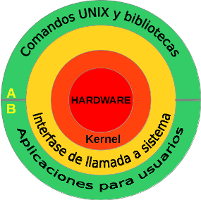
\includegraphics{./img/esquemaOS_s.jpg}
\end{center}

Si un programa es considerado programa de sistema o aplicación 
(A o B en el diagrama), dependerá de su funcionalidad. En apariencia al 
usuario ambos son programas, sin embargo los programas de sistemas son 
útiles a los fines del sistema en si mismo, mientras que las aplicaciones
son útiles a los usuarios. Por ejemplo el programa \texttt{mount} 
\footnote{ Todos los archivos accesible en un sistema UNIX están 
organizados en 
un gran árbol, la jerarquía de archivos cuya raíz es /. Estos 
sistemas de archivos pueden residir en varios dispositivos. El 
comando mount sirve para unir un sistema de archivos ubicado en algún 
dispositivo al árol de directorios principal.Véase \texttt{man mount}}
es un programa de sistema, que puede ser 
utilizado por usuarios administradores, pero que es necesario para el
correcto funcionamiento del sistema. Mientras que un navegador web como 
firefox es una aplicación de usuario. La línea entre uno y otro tipo de 
programas es confusa, sólo nos interesa a fines de comenzar a distinguir
lo que es vital para nuestro sistema de lo que no lo es.  

Los programas de sistema utilizan las herramientas provistas por el
núcleo para implementar varios servicios requeridos en un sistema 
operativo. Los programas de sistema (y todos los demás programas), se 
ejecutan ``por encima del núcleo'', en lo que se denomina 
\textit{modo usuario}. 

Un sistema operativo también puede contener compiladores y sus
correspondientes bibliotecas (GCC y la biblioteca de C en particular para
GNU/Linux), aunque no todos los compiladores de todos los lenguajes de
programación son necesariamente parte del sistema operativo. También 
puede haber documentación, y en algunas ocasiones juegos. 

\subsection{Partes importantes del núcleo}

El núcleo de un sistema GNU/Linux consta de varias partes importantes:
gestión de procesos, gestión de memoria,  controladores para 
dispositivos de hardware, controladores para sistemas de archivos, 
gestión de la red, y otras partes varias. 

 Probablemente las partes más importantes del núcleo (nada funcionaría sin
ellas) son la gestión de memoria y la gestión de procesos. El gestor de 
memoria se encarga de asignar áreas de memoria y de espacio de 
intercambio\footnote{Área de disco utilizada para implementar la memoria 
virtual} a los procesos, partes del núcleo, y también al buffer caché\footnote{http://www.tldp.org/pub/Linux/docs/ldp-archived/system-admin-guide/translations/es/html/ch07s06.html}. El gestor de procesos crea nuevos 
procesos e implementa la multitarea (intercambiando los procesos activos 
en el o los procesadores).

A más bajo nivel, el núcleo contiene un controlador de dispositivo de
hardware para cada tipo de hardware que soporta. Un controlador no es otra
cosa que una pieza de software que sabe cómo ``hablarle'' al dispoitivo en
cuestión, para qué este lleve a cabo su tarea. Debido a que el mundo se
encuentra lleno de diferentes tipos de hardware, el número de 
controladores es grande. Existen frecuentemente, muchas piezas similares 
de hardware que difieren en cómo son controladas por el software. Esta 
singularidad hace posible tener clases generales de controladores que 
soportan operaciones similares; cada miembro de la clase tiene la misma 
interfaz de cara al resto del núcleo pero difiere de los demás miembros 
en la forma de implementar las operaciones. Por
ejemplo, todos los controladores de disco son parecidos para el resto del
núcleo, Por ej., todos tienen operaciones como \textit{iniciar la unidad},
\textit{leer el sector n}, y \textit{escribir en el sector n}.

Algunos servicios de software provistos por el núcleo tienen propiedades
similares, y pueden de esta manera englobarse dentro de clases. Por 
ejemplo, los diferentes protocolos de red fueron englobados dentro de 
una interfaz de programación, la biblioteca de socket BSD. Otro ejemplo 
es la capa del \textit{sistema de archivos virtual} (VFS) que abstrae 
las operaciones de los sistemas de archivos de sus implementaciones. 
Cada tipo de sistema de archivos provee una implementación de cada 
operación. Cuando alguna entidad intenta utilizar un sistema de archivos,
la petición se realiza a través del VFS, el cual la encamina al 
controlador del sistema de archivos correcto.


\subsection{Servicios principales en un sistema UNIX}

 En esta sección se describen brevemente algunos de los servicios más
importantes en un sistema de tipo UNIX.  

\subsubsection{\texttt{\textbf{init}}}

 El servicio individual más importante en un sistema UNIX es provisto por
\texttt{\textbf{init}}. \texttt{\textbf{init}} es el primer proceso que se
inicia en todo sistema UNIX, siendo la última acción que el núcleo 
realiza al arrancar.  Cuando init comienza su ejecución, continúa con el 
proceso de arranque del sistema, realizando varias tareas de inicio 
(chequear y montar sistemas de archivos, iniciar demonios, etc.).  

La lista exacta de cosas que \texttt{\textbf{init}} realiza depende del 
sistema tipo UNIX con el que estemos trabajando. Podemos pensar que init
es quien se encarga de iniciar los programas necesarios para dar 
un determinado grado de funcionalidad al sistema. En este sentidoa, en
principio 
\texttt{\textbf{init}} iniciará un subconjunto de procesos que 
proporciona el concepto de \textit{modo de usuario individual
 (single user mode)}, en el cual nadie, excepto root, puede iniciar una 
sesión; y root utiliza un intérprete de comandos en la consola; este 
modo tiene una funcionalidad reducida y es principalmente utilizado 
para tareas de mantenimiento. Luego, init puede iniciar otro subconjunto 
de funciones adicionales (red, entorno gráfico, etc.) que es conocido 
como \textit{modo multiusuario (multiuser mode)}. En el que múltiples 
usuarios pueden ingresar al sistema simultáneamente.

En general estos modos y otros similares intermedios que puedan exisitr, 
se conocen como \textit{niveles de ejecución (run levels)}. Así, los 
modos individual y multiusuario son considerados dos niveles de ejecución,
y pueden existir otros que identifican un determinado subconjunto de 
funciones. Por ejemplo, podríamos necesitar definir un nivel de ejecución
multiusuario que no inicie el entorno gráfico. 


 GNU/Linux permite tener hasta 10 \textit{niveles de ejecución 
(runlevels)} distintos, numerados de 0-9, pero normalmente solo algunos 
de estos  niveles están definidos de manera predeterminada. El nivel de 
ejecución 0 se define como \textit{sistema detenido (system halt)}. 
El nivel de  ejecución 1 se define como \textit{modo de usuario individual
 (single user mode)}. El nivel de ejecución 6 se define como 
\textit{reinicio del sistema (system reboot)}. Los niveles de ejecución 
restantes dependen de cómo la distribución particular
de GNU/Linux los haya definido, y varían significativamente entre
distribuciones. Observando el contenido del archivo
\texttt{/etc/inittab} podemos hacernos una idea de los niveles de
ejecución preestablecidos en nuestro sistema y de como se encuentran
definidos.

En el funcionamiento normal, \texttt{\textbf{init}} se asegura de que
\texttt{\textbf{getty}} se encuentre trabajando para permitir que los 
usuarios puedan iniciar una sesión, y también se encarga de adoptar 
procesos huérfanos (aquellos cuyo proceso padre murió; en UNIX \textit{todos} los procesos \textit{deben} estar
en un árbol individual, y por esta razón los procesos huérfanos deben ser
adoptados).  

 Al cerrar el sistema, es \texttt{\textbf{init}} quien se encarga de
matar todos los procesos restantes, desmontar todos los sistemas de archivos, y
por último detener el procesador, además de cualquier otra cosa que haya sido
configurado para hacer.  



\subsubsection{Inicio de sesiones desde terminales}

 El inicio de sesiones desde terminales (a través de líneas serie) y la
consola (cuando no se está ejecutando X-Windows) es suministrado por el programa
\texttt{\textbf{getty}}. \texttt{\textbf{init}} inicia una instancia
independiente de \texttt{\textbf{getty}} por cada terminal en el que está permitido iniciar
sesiones. \texttt{\textbf{Getty}} lee el nombre de usuario y ejecuta el
programa login, el cual se encarga de leer la password. Si el nombre de usuario
y la password son correctas, \texttt{\textbf{login}} ejecuta el intérprete de
comandos.  Al finalizar el intérprete de comandos (en el caso en que, por
ejemplo, el usuario finaliza su sesión; o cuando \texttt{\textbf{login}} finaliza debido a que no
concuerdan el nombre de usuario y la password), \texttt{\textbf{init}} se
entera de este suceso e inicia una nueva instancia de \texttt{\textbf{getty}}.
El núcleo no tiene noción sobre los inicios de sesiones, esto es gestionado
totalmente por los \textit{programas del sistema}.  


\subsubsection{Syslog}

 El núcleo y muchos \textit{programas de sistema} producen
mensajes de error, de advertencia y de otros tipos. La mayoría de las veces, es
importante que puedan ser visualizados mas tarde, o tal vez mucho después, por
lo que tales mensajes deben guardarse en un archivo. El programa que realiza
esta tarea es \texttt{\textbf{syslog}}. Syslog puede ser configurado para
ordenar los mensajes en diferentes archivos, de acuerdo a quien lo emite o al
grado de importancia.  Por ejemplo, los mensajes del núcleo son frecuentemente
dirigidos a un archivo separado de los demás, debido a que son más importantes,
y necesitan ser leídos regularmente para detectar problemas.  

\subsubsection{Ejecución periódica de comandos: \texttt{\textbf{cron}} y
\texttt{\textbf{at}}}

 Los administradores de sistemas y los usuarios, a menudo necesitan
ejecutar comandos periódicamente. Como ejemplo, supongamos que el administrador
del sistema desea ejecutar un comando que elimine los archivos más antiguos de
los directorios con archivos temporales (\texttt{/tmp} y
\texttt{/var/tmp}) para evitar así que el disco se llene, debido a
que no todos los programas eliminan correctamente los archivos temporales que
ellos mismos generan.  

 El servicio \texttt{\textbf{cron}} se configura para que realice la
tarea anterior. Cada usuario tiene un archivo \texttt{crontab}, en
el cual se listan los comandos que se desea ejecutar y la fecha y hora de
ejecución. El servicio \texttt{\textbf{cron}} se encarga con precisión de
iniciar cada comando, a la fecha y hora adecuada de acuerdo a lo especificado en
cada archivo crontab.  

 El servicio \texttt{\textbf{at}} es similar a \texttt{\textbf{cron}},
pero este se inicia únicamente una vez: el comando es ejecutado a la hora
especificada, pero esta ejecución no vuelve a repetirse.  

 Se puede encontrar información adicional sobre cron(1), crontab(5), at(1)
y atd(8) en las páginas de manual.  

\subsubsection{ Interfaz gráfica de usuario (GUI)}

 UNIX y GNU/Linux no incorporan la interfaz gráfica de usuario dentro del
núcleo; en su lugar, es implementada por programas a nivel de usuario. Esto se
aplica tanto a entornos gráficos como al modo texto.  

 Esta disposición hace que el sistema sea más flexible, pero tiene la
desventaja de que, al ser simple implementar una interfaz de usuario diferente
para cada programa, dificulta el aprendizaje del sistema.  

 El entorno gráfico principalmente utilizado con GNU/Linux se llama
Sistema X-Windows (X para abreviar). X tampoco implementa por sí mismo una
interfaz de usuario, sino solo un sistema de ventanas. Es decir, las
herramientas base con las cuales se puede construir una interfaz gráfica de
usuario. Algunos administradores de ventanas populares son: fvwm, icewm,
blackbox y metacity. Existen también dos populares administradores de
escritorios: KDE y Gnome.  


\subsubsection{ Redes}

 Una red se construye al conectar dos o más computadoras para que puedan
comunicarse entre sí. Los métodos actuales de conexión y comunicación son
ligeramente complicados, pero el resultado final es muy útil.  

 Los sistemas operativos UNIX tienen un diseño orientado hacia el uso 
de red. La mayoría de los servicios básicos (sistemas de archivos, impresión, 
copias de seguridad, etc) pueden utilizarse a través de la red. Aprovechar estas
características puede ayudar a que la administración del sistema sea más fácil. 
Por ejemplo permite tener una administración centralizada de impresoras, recolección 
de logs, sistemas de copia de respaldo, evitar la duplicación 
de archivos mediante sistemas de archivos en red (véase NFS), etc.

 Este apunte de cátedra sólo aborda superficialmente la teoría de
redes. Información adicional sobre esteos tema será desarrollada en la materia 
``Redes'', dedicada a tal fin. Adicionalmente puede consultar ``La Guía De Administración 
De Redes con Linux'' (\textit{Linux Network Administrators' Guide} 
\footnote{	http://www.tldp.org/LDP/nag2/index.html}
incluyendo una descripción básica de como
operan las redes.  

\subsubsection{ Inicio de sesiones a través de la red}

 Los inicios de sesión a través de la red funcionan de un modo un poco
diferente al inicio de sesiones normales. En cuyo caso existe una línea serie 
física separada para cada terminal a través de la cual es posible iniciar sesión. 
Por cada persona iniciando una sesión a través de la red existe una conexión de red
virtual, y puede haber cualquier número (no hay límite).  
\footnote{Al menos puede haber muchas. Dado que el ancho de banda es un
recurso escaso, existe aún en la práctica algún límite al
número de inicios de sesión concurrentes a través de una conexión
de red. }

Por lo tanto, no es posible ejecutar \texttt{\textbf{getty}} por separado 
por cada conexión virtual posible. Existen
también varias maneras diferentes de iniciar una sesión a través de la red, las
principales en redes TCP/IP son \texttt{\textbf{telnet}} y \texttt{\textbf{ssh}}.
\footnote{El programa \texttt{\textbf{telnet}} implementa toda la comunicación basado en
texto plano (sin cifrar), exponiendo así nombre de usuarios, contraseñas y otro tipo de 
información sensible, a potenciales intrusos que se encuentren observando el tráfico en la red. 
En su lugar, y siempre que sea posible, es recomendable utilizar el programa \texttt{\textbf{ssh }}, 
\textit{intérprete de comandos seguro} que cifra el tráfico en la red, haciendo
así bastante menos probable el robo de información}


 Los inicios de sesión a través de la red tienen, en vez de una cantidad
enorme de \texttt{\textbf{getty's}}, un servicio individual por tipo de 
inicio de sesión (\texttt{\textbf{telnet}} y \texttt{\textbf{ssh}}
tienen servicios separados) que \textit{escucha} todos los intentos de inicio de
sesión entrantes. Cuando el servicio advierte un intento de inicio de sesión,
inicia una nueva instancia de si mismo para atender la petición individual; la
instancia original continúa atenta a otros posibles intentos. La nueva instancia
trabaja de manera similar a \texttt{\textbf{getty}}.  


\subsubsection{ Sistemas de archivos de red (NFS)}  

Una de las cosas
más útiles que se pueden hacer con los servicios de red es compartir archivos a
través de un \textit{sistema de archivos de red}. El más utilizado
normalmente para compartir archivos se llama \textit{Network File
System}, o \textit{NFS}, desarrollado por Sun Microsystems (actualmente Oracle).  

 Con un sistema de archivos de red, cualquier operación sobre un archivo
realizada por un programa en una máquina es enviada a través de la red a otra
máquina. Se \textit{engaña} al programa, haciéndole creer que todos los archivos en la
computadora remota se encuentran de hecho en la computadora en el que el programa se
está ejecutando. Con esta manera de trabajar, compartir información es
extremadamente simple, ya que no se requieren modificaciones en el programa.


 Otra manera muy popular de compartir archivos es a través de Samba
(http://www.samba.org). Este protocolo
(llamado SMB) permite compartir archivos con máquinas con sistema oeprativo
Windows(c) a través del Entorno de Red. También permite compartir impresoras.  


\subsubsection{ Correo}

 El correo electrónico es el método más popularmente utilizado para
comunicarse a través de la computadora. Una carta electrónica (email) se almacena en un
archivo con un formato especial, y se utilizan programas de correo especiales
para enviar y leer las cartas (emails).  

 Cada usuario tiene un \textit{buzón de correo entrante} (un
archivo con formato especial), en donde se almacena todo el correo nuevo. Cuando
alguien  envía un correo, el programa de correo localiza el buzón del
destinatario y agrega la carta al archivo de buzón de correo entrante. Si el
buzón del destinatario se encuentra en otra máquina, la carta es enviada allí,
donde se traslada al buzón de correo como corresponda.  

 El sistema de correo se compone de muchos programas. El transporte del
correo a buzones locales o remotos es realizado por un programa: \textit{el
agente de transporte de correo} o \textit{MTA}.
(\texttt{\textbf{Sendmail}}, \texttt{\textbf{Postfix}} y \texttt{\textbf{Exim}} son ejemplos de
esto), mientras que existe un sin número de programas muy variados que los
usuarios utilizan para leer y escribir correos. \textit{Estos son conocidos
como agentes de usuario de correo }o \textit{MUA},
(\texttt{\textbf{mailx}} y \texttt{\textbf{Thunderbird}} son ejemplos de esto). Los
archivos de buzones de correo están usualmente ubicados en
\texttt{/var/spool/mail}.  



\subsubsection{Impresión}

 Sólo una persona puede utilizar la impresora en un momento, pero
sería antieconómico no compartir impresoras entre los usuarios. La impresora es
por lo tanto administrada por software que implementa una cola de impresión:
todos los trabajos de impresión son colocados dentro de la cola, y una vez que
la impresora termina de imprimir una trabajo, el siguiente es enviado a la
impresora automáticamente. Esto alivia al usuario de la organización de la cola
de impresión y de luchar por el control de la impresora.  

 El software de la cola de impresión también coloca los trabajos de
impresión en disco, es decir, el texto a imprimir es mantenido en un archivo
mientras que el trabajo se encuentre en la cola. Esto permite a los programas de
aplicación entregar rápidamente los trabajos a imprimir al software que
administra la \textit{cola de impresión}; así, las aplicaciones no
tienen que esperar a que el trabajo (en inglés \textit{job}) esté de hecho impreso para
poder continuar su ejecución. Esta forma de trabajar es realmente cómoda, ya que
permite enviar a imprimir una versión de un trabajo y no tener que esperar a que
ésta sea impresa antes de poder hacer una versión nueva completamente revisada.


\fcolorbox{black}{grey}{
\parbox[t]{1.0\linewidth}{ \vspace*{0.4cm}
El servicio de impresión mas utilizado en los sistemas GNU/Linux
es \textbf{CUPS}. \textbf{CUPS} es un sistema de impresión open source
desarrollado por Apple(c) para sistemas UNIX \textbf{\texttt{http://www.cups.org}}
\vspace*{0.4cm} } }


\subsubsection{ La distribución del sistema de archivos}



 El sistema de archivos está dividido en muchas partes, las cuáles pueden residir
en lugares físicos diversos; normalmente en un sistema de archivos raíz podremos 
encontrar el directorio \texttt{/bin}, \texttt{/lib}, \texttt{/etc}, \texttt{/dev},
y otros pocos directorios; un sistema de archivos \texttt{/usr} con programas y datos que
no tendrán cambios; un sistema de archivos \texttt{/var} con datos que pueden cambiar
(como los archivos de log); y un sistema de archivos \texttt{/home}
para todos los archivos personales de los usuarios. Dependiendo de la
configuración del hardware y de las decisiones del administrador del sistema, la
división puede llegar a ser diferente; a pesar de esto, y aunque la división es
aconsejable, es también posible distribuir todos los archivos en un solo sistema
de archivos.  

 En el apunte de cátedra referente al árbol de directorios se detallaran más 
aspectos acerca de la distribución del sistema de archivos. Si desea más información,
también puede consultar el documento \textit{Estándar de la Jerarquía del Sistema de Archivos
de Linux} 
\footnote{http://www.linuxfoundation.org/collaborate/workgroups/lsb/fhs}
que cubre este tema en profundidad, o bien la página del manual en línea hier (7).

\section*{Licencia}
This is a derived version of "Guía Para Administradores de Sistemas GNU/Linux" that 
can be found at \\ \texttt{http://www.ibiblio.org/pub/Linux/docs/LDP/system-admin-guide/translations/es/gasl.txt}.

Copyright (C) 1993-1998 Lars Wirzenius.

Copyright (C) 1998-2001 Joanna Oja.

Copyright (C) 2001-2003 Stephen Stafford.

Copyright (C) 2003-2004 Stephen Stafford and Alex Weeks.

Copyright (C) 2004-Present Alex Weeks.

Copyright (C) 2013-Present Rafael Ignacio Zurita

Trademarks are owned by their owners.

Permission is granted to copy, distribute and/or modify this document under
the terms of the GNU Free Documentation License, Version 1.2 or any later
version published by the Free Software Foundation; with no Invariant
Sections, no Front-Cover Texts, and no Back-Cover Texts. A copy of the
license is included in the section entitled "GNU Free Documentation License".

\subsection*{Traducción de la licencia}
Esta es una obra derivada de "Guía Para Administradores de Sistemas GNU/Linux" que puede 
econtrarse en \\ \texttt{http://www.ibiblio.org/pub/Linux/docs/LDP/system-admin-guide/translations/es/gasl.txt}.

Las marcas registradas son propiedad de sus dueños.

Se concede autorización para copiar, distribuir y/o modificar este documento
bajo los términos de la Licencia de documentación libre GNU (FDL), Versión 1.2; 
sin Secciones Invariantes, sin textos de Portada, y sin Textos de Contra Portada. 
Una copia de la licencia se encuentra incluída en la sección "GNU Free Documentation License".


\end{document}
